% vim: tw=80 sw=2 ts=2 ff=unix spelllang=en spell
\documentclass{beamer}
\newcommand{\colA}[1]{\begin{columns}[t]\begin{column}{#1}}
\newcommand{\colB}[1]{\end{column}\begin{column}{#1}}
\newcommand{\colEnd}{\end{column}\end{columns}}

\usetheme{CambridgeUS}
\usecolortheme{dolphin}
%\setbeamercovered{transparent}
%\useoutertheme{infolines}

\usepackage{xltxtra}
\usepackage{fancyvrb}
%% \usepackage{ngerman}
\institute[]{Centrum für Informations- und Sprachverarbeitung (CIS)\\
            Ludwig-Maximilians-Universität München (LMU)\\
            \vspace{1cm}
            \href{https://creativecommons.org/licenses/by-nc-sa/4.0/}%
            {\includegraphics[width=0.2\textwidth]{../presentations/images/by-nc-sa.eps}}}

% keine Navigationspfeile
\setbeamertemplate{navigation symbols}{} % keine Navigations-Buttons

% Standardschrift verändern für Griechisch
%\setsansfont[Mapping=tex-text]{Junicode}
%\setmonofont[Mapping=tex-text]{DejaVu Sans Mono}
%\setsansfont[Mapping=tex-text]{Linux Libertine O}
%\setsansfont[Scale=MatchLowercase]{Linux Biolinum O}

% Fußzeile mit Titel und Seitenr.
\definecolor{mygray}{gray}{0.25}
%\setbeamertemplate{footline}[frame number]
\setbeamertemplate{footline}{\color{mygray}\hspace*{2mm}\insertauthor\hfill \insertshorttitle\hfill\insertdate\hspace*{10pt}\insertframenumber\ / \inserttotalframenumber\hspace*{2ex}}

% Schrift für URLs
\definecolor{myblue}{rgb}{0.2 0.0 0.8}

\usepackage{hyperref}
\renewcommand{\UrlFont}{\color{myblue}\footnotesize\sf}
\hypersetup{colorlinks,allcolors=.,urlcolor=blue}

% Bibliography
%\usepackage[backend=biber,style=authoryear,maxcitenames=2,maxbibnames=9]{biblatex}

% Schriftgröße Listings
\RequirePackage{fancyvrb}
\DefineVerbatimEnvironment{Highlighting}{Verbatim}%
  {commandchars=\\\{\},fontsize=\footnotesize}
\DefineVerbatimEnvironment{Verbatim}{Verbatim}%
  {fontsize=\footnotesize}
\newcommand{\pocoto}{\texttt{PoCoTo}}

\title{DATeCH 2017 -- \pocoto{} Workshop -- Profiler}
\author{Florian~Fink \& Uwe~Springmann}

\begin{document}

\begin{frame}
	\titlepage
\end{frame}

\section{Profiling}
\subsection{Overview}
\begin{frame}
	\begin{itemize}
		\item OCR'ed historical Documents contain errors.
		\item Historical documents contain lots of spelling variation.
		\item If you want to find errors in OCR'ed documents, you need a fitting
			historical dictionary.
		\item If you only have a modern dictionary, you will get a lot of false
			positives (\emph{vnnd}, \emph{Thurm}, \dots).
	\end{itemize}
\end{frame}

\subsection{Language profiler}
\begin{frame}
	The language Profiler was created to help to find OCR-errors in OCR'ed
	historical documents and to generate correction candidates for suspected
	errors\footnote{Ulrich Reffle, \emph{Algorithmen und Methoden zur
	dokumentenspezifischen Analyse historischer und OCR-erfasster Texte}, 2011}.

	\begin{itemize}
		\item The profiler tries to distinguish real OCR-errors from historical
			spelling variants.
		\item The profiler can detect OCR-errors in historical patterns.
		\item The profiler uses various modern dictionaries.
		\item The profiler uses a pattern list, that describes
			historical spelling variations.
		\item The profiler generates a document-dependent error profile (the
			\emph{document profile}).% that uses an expectation maximization algorithm
			to maximize the
			%probabilities of the OCR and language patterns for a given document.
	\end{itemize}
\end{frame}

\section{Profiler}
\subsection{Documentation}
\begin{frame}
	\begin{itemize}
		\item The profiler is documented in the
			\href{https://github.com/cisocrgroup/Resources/blob/master/manuals/profiler-manual.pdf}{profiler
			manual} (included in the workshop's data package).
		\item Its source is available on \href{https://github.com/cisocrgroup/Profiler}{github}.
		\item The profiling web service, that is used by \pocoto{} is also available
			on \href{https://github.com/cisocrgroup/ProfilerWebService}{github}.
		\item It needs Linux and different C++ development tools (cmake, make, g++,
			boost, xerces, \dots).
		\item The profiler contains various tools that compile different forms of
			dictionaries, perform lookup in different dictionaries and generate
			correction candidates for unknown words.
	\end{itemize}
\end{frame}

\subsection{Language back-end}
\begin{frame}
	The profiler uses a so called \emph{language back-end}, that contains the
	language dependent resources for the profiler. A minimal language back-end
	contains at least:
	\begin{itemize}
		\item A configuration file
		\item A compiled modern dictionary.
		\item A historical pattern file \item A frequency list of a historical
			patterns from a ground truth\footnote{This is a bug, since this resource
			should be purely optional.}
	\end{itemize}
\end{frame}

\subsection{Resources}
\begin{frame}
	\begin{itemize}
		\item Dictionaries must be compiled from plain text files using the
			\texttt{compileFBDic}.
		\item The historical pattern file is a plain text file that lists various
			spelling variation patterns in the form: \texttt{modern:historical}.
		\item The frequency list must be compiled from a historical ground truth
			using the \texttt{trainFrequencyList} tool\footnote{You can use a small
			garbage file if you do not have a appropriate historical ground truth.}
	\end{itemize}
\end{frame}

\subsection{Configuration file}
\begin{frame}
	\begin{itemize}
		\item The configuration file sets some variables for the profiler.
		\item Its main purpose is to set up the profiling process.
		\item It defines which pattern file to use
		\item It defines the dictionaries to use and the order of their evaluation.
		\item There is a simple configuration file on
			\href{https://github.com/cisocrgroup/Resources/blob/master/lexica/german.ini}{github}.
	\end{itemize}
\end{frame}

%\subsecion{Example configuration file}
\begin{frame}[fragile]
	\begin{Verbatim}[fontsize=\small]
...
# Dictionary and Pattern settings
[language_model]
patternFile = "${:PATH}/patterns.txt"
...
# RANK 0
[dict_modernExact]
path = "${:PATH}/modern.fbdic"
histPatterns = 0
ocrErrors = 0
ocrErrorsOnHypothetic = 0
cascadeRank = 0
# RANK 2
[dict_modernHypotheticError]
path = "${:PATH}/modern.fbdic"
histPatterns = 3
ocrErrors = 2
ocrErrorsOnHypothetic = 1
cascadeRank = 2
	\end{Verbatim}
\end{frame}

\subsection{Pattern file}
\begin{frame}
	\begin{itemize}
		\item If you work with the profiler you will often recognize missing
			historical patterns.
		\item The simplest resource to update is the historical pattern list.
		\item It is a plain text file that can be edited.
		\item New patterns can be added easily to the pattern file.
		\item There are some example pattern files on
			\href{https://github.com/cisocrgroup/Resources/tree/master/lexica}{github}.
	\end{itemize}
\end{frame}

\subsection{Example pattern file}
\begin{frame}[fragile]
	The pattern file is a plain text file with one pattern per line. Each pattern
	must be of the form \texttt{modern:hist}. You can use \texttt{\$} to mark end
	of words. Lines that start with \texttt{\#} are ignored:

\begin{verbatim}
# patterns.txt
# cases are ignored!
# turm was often spelled thurm
t:th
# teil was often spelled theyl
ei:ey
# $ marks the end of words
lich$:lig$
bar$:lich$
\end{verbatim}
\end{frame}

\subsection{Dictionaries}
\begin{frame}
	\begin{itemize}
		\item Dictionaries are compiled from plain text files.
		\item Each token is on its own line.
		\item The text files must be sorted in ascending order.
		\item To add entries to a dictionary, you
			\begin{itemize}
				\item add the dictionary entry to the file
				\item sort the file
				\item compile the dictionary from the sorted file
			\end{itemize}
		\item There are some example dictionaries on
			\href{https://github.com/cisocrgroup/Resources/tree/master/lexica}{github}.
	\end{itemize}
\end{frame}

\section{Profiling documents}
\subsection{Minimal language back-end}
\begin{frame}[fragile]
\begin{Verbatim}
+-- my-language
|   +-- freqlist.binfrq
|   +-- modern.fbdic
|   +-- patterns.txt
|   +-- weights.txt
+-- my-language.ini
\end{Verbatim}
	\begin{itemize}
		\item With the profiler you can now profile your own documents.
		\item First of all you need a minimal language back-end.
		\item The language back-end contains at least:
			\begin{itemize}
				\item A configuration file
				\item A compiled modern dictionary
				\item A pattern file
				\item Two files that describe the historical ground truth
					(\texttt{weights.txt}, \texttt{freqlist.binfrq})
			\end{itemize}
	\end{itemize}
\end{frame}

\subsection{Manual profiling}
\begin{frame}
	\begin{itemize}
		\item The profiler can profile plain text or \texttt{DocXML}
			documents.
		\item The command \texttt{profiler --config my-language.ini --sourceFile my-doc.xml
			--out\_xml patterns.xml --out\_doc my-doc-out.xml} starts the profiling.
		\item The profiler produces two output files:
			\begin{enumerate}
				\item \texttt{patterns.xml} lists the assumed historical and OCR-error
					patterns and their occurrences in the document.
				\item \texttt{my-doc-out.xml} contains a \texttt{DocXML} file with
					correction suggestions for the unknown tokens.
			\end{enumerate}
		\item The profiler has some more command options (\texttt{profiler --help}).
	\end{itemize}
\end{frame}

\subsection{Correction candidates I}
\begin{frame}[fragile]
	\begin{verbatim}
<token token_id="16" isNormal="true">
  <ext_id>16</ext_id>
  <wOCR>vber</wOCR>
  <wOCR_lc>vber</wOCR_lc>
  <wCorr></wCorr>
  <cand>vber:{über+[(ü:v,0)]}+ocr[],voteWeight=0.9503,
    levDistance=0</cand>
  <cand>über:{über+[]}+ocr[(ü:v,0)],voteWeight=0.0489158,
    levDistance=1</cand>
  <cand>uber:{über+[(ü:u,0)]}+ocr[(u:v,0)],voteWeight=0.00...
    levDistance=1</cand>
  <!-- ... -->
</token>
\end{verbatim}
\end{frame}

\subsection{Correction candidates II}
\begin{frame}[fragile]
	\begin{Verbatim}[fontsize=\small]
(ocr:vber)
uber:{über+[(ü:u,0)]}+ocr[(u:v,0)]
^     ^      ^   ^         ^   ^
|     |      |   |         |   |
|     |      |   |         |   +- error pattern position
|     |      |   |         + ---- error pattern (correct:ocr)
|     |      |   +--------------- hist pattern position
|     |      +------------------- hist pattern (mod:hist)
|     +-------------------------- correct modern version
+-------------------------------- correction candidate
\end{Verbatim}
\end{frame}

\section{Profiling with \pocoto}
\subsection{Profiling web-service}
\begin{frame}
	\begin{itemize}
		\item The profiler web-service is a wrapper around the profiler with various
			language back-ends.
		\item It offers a SOAP-based web interface to profile documents.
		\item Its documentation is in the
			\href{https://github.com/cisocrgroup/Resources/blob/master/manuals/profiler-manual.pdf}{profiler manual}
		\item Its source code is on
			\href{https://github.com/cisocrgroup/ProfilerWebService}{github}.
		\item \pocoto{} can connect to such a web-service to profile a document.
	\end{itemize}
\end{frame}


\subsection{Configuring the web-service}
\begin{frame}
	\begin{itemize}
		\item You can configure the URL of the web-service going to
			\texttt{Tools->Options->Profiler}
		\item The default URL points to a profiling web-service hosted by CLARIN-D.
		\item The CLARIN-D web-service has language-back-ends for German, Latin and
			Greek.
	\end{itemize}
\end{frame}

\subsection{Profiling a project with the profiling web-service}
\begin{frame}
	\begin{itemize}
		\item You can profile your current project by clicking
			\texttt{Profiler->Order document profiler} in the menu area.
		\item You will be asked which language back-end to use
		\item Select a language and click \texttt{Order document profile}.
		\item depending on your document and the settings of the profiler the
			profiling can take some time.
		\item After the profiling has stopped, you now will have access to the
			common error pattern tab in the error area and you will get a list of
			correction suggestions if you try to correct a token.
	\end{itemize}
\end{frame}

\subsection{Profiling with a custom profiler}
\begin{frame}
		If the profiler web-service does not support your language or if you want to
		improve the language resources, you can profile the document manually and
		import it back into \pocoto{}.
	\begin{enumerate}
		\item Export your project \texttt{File->Export->Export as DocXML}.
		\item Run the profiler on the \texttt{DocXML} file.
		\item Import the two output files of the profiler back into \pocoto{}.
	\end{enumerate}
\end{frame}

\section{}
\subsection{}
\begin{frame}
	\centering{
		\Huge Thanks for your attention!
	}
\end{frame}

\end{document}

